The \emph{image\_recognition} packages apply state of the art image classification techniques based on \acrfull{cnn}.

%\begin{figure}[H]
%    \centering
%    \vspace{-1em}
%	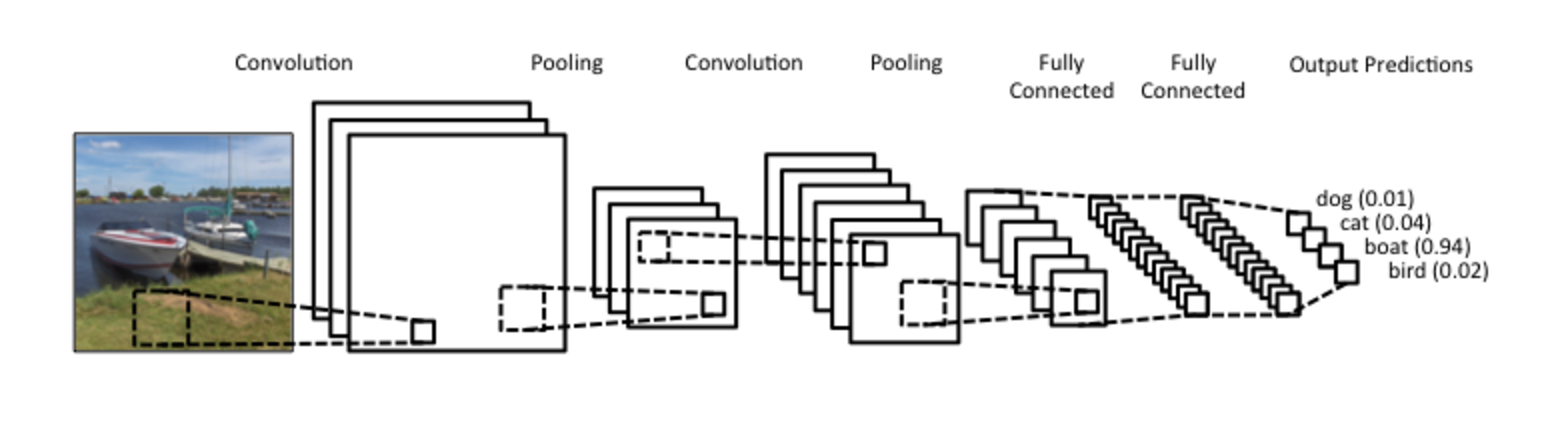
\includegraphics[width = 1\linewidth]{Figures/cnn}
%    %\vspace{-1em}
%    \caption{Illustration of \acrfull{cnn} used in our object recognition %nodes with use of Tensorflow.}
%	\label{fig:cnn}
%    %\vspace{-0.5cm}
%\end{figure}

\begin{enumerate}
\item \textbf{Object recognition:} Tensorflow\texttrademark\hspace{0em} with retrained top-layer of a Inception V3 neural network.
%, as illustrated in Figure \ref{fig:cnn}.
%The top layers are retrained on a custom dataset using a soft-max top-layer that maps the image representation on a specified set of labels.
%\\
%In order to create a new training set for specific objects the \emph{image\_recognition} packages contain several tools for annotating objects.
%Tools for retraining neural networks are also included.

\item \textbf{Face recognition:} OpenFace\footnote{\url{https://cmusatyalab.github.io/openface/}}, based on Torch.
%OpenFace is an existing state-of-the-art face recognition library. We implemented a ROS node that enables the use of these advanced technologies within the ROS network.

\item \textbf{Pose detection:} OpenPose\footnote{\url{https://github.com/CMU-Perceptual-Computing-Lab/openpose}}.
\end{enumerate}
%\subsection{ROS packages}
%Our image recognition ROS packages can be found on GitHub\footnote{\url{https://github.com/tue-robotics/image_recognition}} together with tutorials and documentation.
%Recently, they have also been added to the ROS Kinetic package list and can be installed as Debian packages: \emph{ros-kinetic-image-recognition}
Our image recognition ROS packages are available on GitHub\footnote{\url{https://github.com/tue-robotics/image_recognition}} and as Debian packages: \emph{ros-noetic-image-recognition}.
Our ongoing efforts are to upgrade these to a YOLOv8 based pipeline for object recognition and pose detection, and FaceNet for face recognition, all implement in PyTorch 2.1 with TensorRT.